\section{Isolated Quantum Dot}
\subsection{Engineering the spectrum}\label{subsec:spectrum_engineering}

To encourage impact ionisation, we engineer the quantum dot to have 4 equally spaced energy levels. As shown in Fig. \ref{fig:qd_spectrum_delta} (and Fig \ref{fig:impact_ionisation}) this allows for an electron from the lower Hubbard band to be excited into the most energetic state and during its subsequent decay, to promote a second electron over the Mott gap.
\newline
%{\color{red} do the lines represent states of electrons or states of the entire system?}

\begin{figure}[!hbt]
    \centering
    \begin{tikzpicture}[eline/.style={ultra thick, black},
                        earrow/.style={->, >=Latex, thick, shorten >=3pt, shorten <=3pt},
                        squiggly/.style={->, thick, decorate, decoration=snake, yellow!70!red}
                        ]
        
     
        \newdimen\height
        \height = 2.5cm
        \newdimen\baselength
        \baselength = 4cm
        \newdimen\arrowgap
        \arrowgap = 0.25cm
        
         % draw E axis and make nodes for energy levels
        \draw[->,>=stealth, ultra thick, black!50] ($(-\baselength,0)/2$) -- ($(\baselength,0)/2$) 
                                                    node[pos=0.5, inner sep=0, label=below:{\tiny E$_{\mathrm F}$}] (EF){}
                                                    node[pos=0.2, inner sep=0] (E1){}
                                                    node[pos=0.4, inner sep=0] (E2){}
                                                    node[pos=0.6, inner sep=0] (E3){}
                                                    node[pos=0.8, inner sep=0] (E4){}
                                                    node[pos=1, anchor=north]{\small E};
                                                            
        % tick for fermi energy
        \draw[thick, black!50] ($(EF) + (0,-3pt)$) -- ($(EF) + (0,3pt)$);
        
        % energy lines
        \foreach \i in {1, 2, 3, 4} 
        \draw[eline] (E\i) -- ($(E\i)+(0,\height)$) node[pos=0.5, inner sep=0] (halfE\i){};
        
        % electron transition lines
        % 1st arrow
        \draw[earrow, red]     ($(halfE2.west)+(0,\arrowgap)$) to [out = 30, in=150] 
                                node[pos=0.8, inner sep=1pt, outer sep=4pt, anchor=south, circle, draw]{\tiny$1$}
                                ($(halfE4.east)+(0,\arrowgap)$);
                                
        % impact io arrows
        \draw[earrow, black!60]     ($(halfE2.west)-(0,\arrowgap)$) to [out = 30, in= 150]  
                                node[pos=0.5, inner sep=0] (halfE23) {} 
                                ($(halfE3.east)-(0,\arrowgap)$);
                                
        \draw[earrow, black!60]     ($(halfE4.east)-(0,\arrowgap)$) to [out =-150, in=-30]  
                                node[pos=0.5, inner sep=0] (halfE43) {} 
                                node[pos=0.7, inner sep=1pt, outer sep=4pt, anchor=south, circle, draw]{\tiny$2$}
                                ($(halfE3.west)-(0,\arrowgap)$);
                               
        
        % squiggly line
        \draw[squiggly] (halfE43) to[out=-120, in=-80] (halfE23);
        
    \end{tikzpicture}
    \captionsetup{singlelinecheck=off}
    \caption{Illustration of why equally spaced energy levels encourage impact ionisation.
    \newline
    1. An electron is promoted by two energy levels. 
    \newline
    2. The promoted electron gives up half its energy to promote a second electron}
    \label{fig:qd_spectrum_delta}
\end{figure}

The main parameter that needs to be tuned to achieve such a spectrum is the on site coulomb potential $U \equiv U_{ii}$, as it is directly responsible for the size of the Mott gap. A loop was set up to compute the Lehmann spectrum of the system for a range of values of $U$. The mean differences in the spacings between the peaks were extracted and plotted as a function of the coulomb potential. By regressing a line to this data we were then able to determine that for our choice of parameters, $U = 2.41$ produced the desired energy level spacing. Fig. \ref{fig:spectrum_engineering} shows a series of Lehmann spectra that were produced in this process as well as the final, equally spaced spectrum.


\begin{figure}[!hbt]
    \centering
    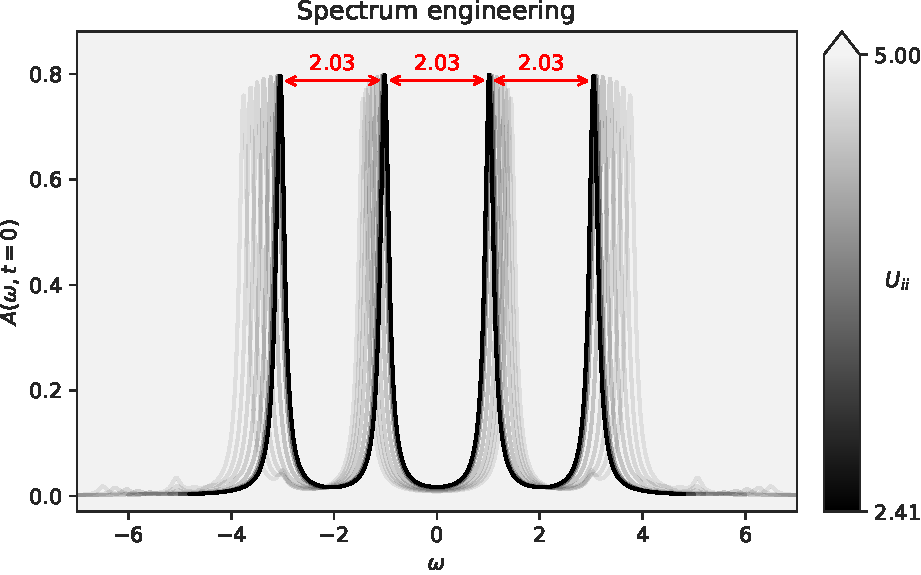
\includegraphics[width=0.7\textwidth]{graph/spectrum_engineering.pdf}
    \caption{temporary. Lehmann spectrum taken on site 0, but looks the same on all sites. if it matters black to white transition can be improved}
    \label{fig:spectrum_engineering}
\end{figure}

\subsection{Not seeing transition at expected energie, ie. why spectral function may be bad for small systems}
In Fig. \ref{fig:qd_9_total_energy} we see the Total energy of the spectrum engineered QD over time, after being subjected to a light pulse of varying frequencies $\omega$. As expected, for low values of $\omega$ no electrons can be excited over the Mott gap and thus no energy from the light pulse is absorbed. At $\omega = 2.00$ we see an energy increase as the light is now energetic enough to promote an electron into the upper hubbard band.

\medskip

Rather unexpectedly however, we see no energy gain at $\omega = 4.00$, meaning the first transition shown in Fig. \ref{fig:qd_spectrum_delta} seems to not be taking place.

\medskip

One possible explanation for this may be that the spectral functions we are using are not truly representative of the transitions between the eigenstates of our system. As briefly explained in section \ref{sec:spectral_functions}, we compute spectral functions by adding an electron/hole to the system, letting it propagate for a fixed time, then removing it again, and evaluating the overlap of this system with an unmodified one. Thus the spectral function shows us transitions between systems with electron numbers differing by one. For large systems, with many electrons, adding or removing a single electron has an insignificant effect on its eigenenergy spectrum and thus it will be equal to the spectral function. However, for a small 2x2 site system like our QD, the effect may no longer be negligible. Meaning that the spectrum we see in Fig. \ref{fig:spectrum_engineering} may not accurately represent the true eigenenergies of the QD and the transition at $\omega\approx 4$ may not be possible.

\medskip
It may be possible to remedy this with the use of Loschmid spectra, which do not suffer from the same issues in small systems ({\color{red} I should probably cite something here about Loschmid spectra. What about this: \cite{loschmidt}?}). However the implementation of these will have to wait for a future project. 

\medskip

\begin{figure}[!hbt]
    \centering
    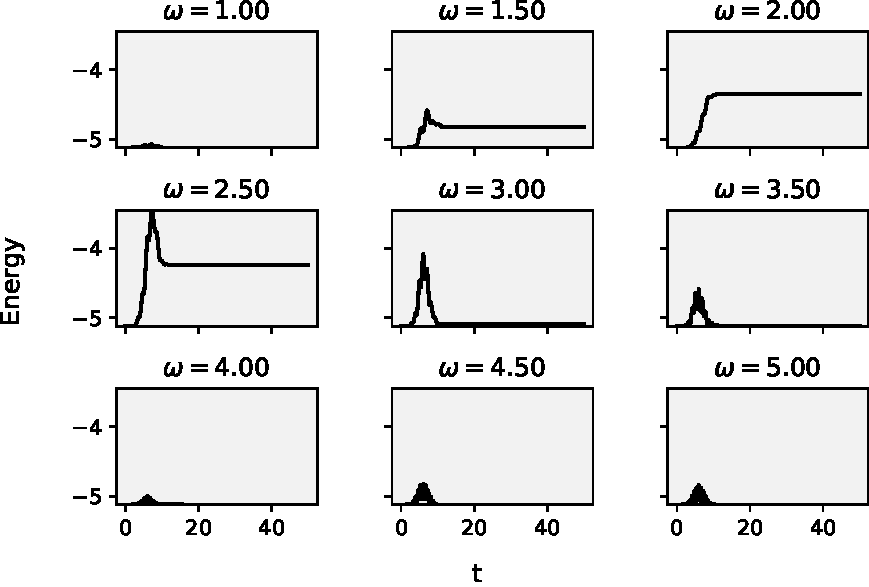
\includegraphics[width=0.7\textwidth]{graph/9test.pdf}
    \caption{Total energy in isolated QD system after interaction with light pulse at $t=6$ for various frequencies $\omega$.}
    \label{fig:qd_9_total_energy}
\end{figure}